\documentclass{article}

\usepackage{graphicx} % more modern
\usepackage{subcaption} 

% For citations
\usepackage{natbib}
\usepackage{url}

% For algorithms
\usepackage{algorithm}
\usepackage{algorithmic}
\usepackage{hyperref}
\usepackage{booktabs}
\usepackage{multirow}
\usepackage{amsmath}

\usepackage{array}

% \usepackage{dblfloatfix}
% \usepackage{fixltx2e}


\usepackage[accepted]{icml2017}

\def\docTitle{Inception U-Net: Ultrasound Nerve Segmentation}

\icmltitlerunning{\docTitle}
\title{Inception U-Net}

\begin{document} 

\twocolumn[
\icmltitle{\docTitle}

% It is OKAY to include author information, even for blind
% submissions: the style file will automatically remove it for you
% unless you've provided the [accepted] option to the icml2013
% package.

\begin{icmlauthorlist}
\icmlauthor{Peter James Bernante}{cs} \\
{\tt\small Maharishi University of Management} \\
{\tt\small pjbernante@mum.edu}
\end{icmlauthorlist}

\icmlaffiliation{cs}{Computer Science Department, Maharishi University of Management, Iowa, USA}

\icmlcorrespondingauthor{Peter James Bernante}{pjbernante@mum.edu}

% You may provide any keywords that you 
% find helpful for describing your paper; these are used to populate 
% the "keywords" metadata in the PDF but will not be shown in the document
\icmlkeywords{healthcare, medical imaging, convolutional neural networks, ultrasound, brachial plexus, nerve segmentation, segmentation}
\vskip 0.3in

\begin{abstract}
We develop an algorithm that can detect a collection of nerve structures called the Brachial Plexus (BP) \cite{wiki:Brachial_plexus}.
Our algorithm, Inception U-Net, is a deep convolutional neural network trained on ultrasound images from \cite{kaggle:ultrasound-nerve-segmentation}. The images were manually annotated by humans who were experts. We used a modified U-Net \cite{2015arXiv150504597R} architecture, and replaced its VGG-like \cite{2014arXiv1409.1556S} layers with Inception Modules \cite{2015arXiv151200567S}. We find that the Inception Modules made the model deeper and significantly reduced the number of parameters. We also found that, although the number of parameters is only a fraction of the standard U-Net, it had better performance in terms of defined metrics. Our algorithm was also able to annotate the images where the human annotators could not.
\end{abstract}
\bigskip
]
\printAffiliationsAndNotice{}

\section{Introduction}
Surgery oftentimes involves post-surgical pain. Managing pain involves the use of narcotics which have several unwanted side effects; under or overdosing respiratory side effects and sedation.

One way to manage pain with less dependency on narcotics is through the use of indwelling catheters that deliver anesthetic. Pain management catheters block or mitigate the pain at the source. These catheters are inserted in the area around the nerves that carries sensation from the surgical site. It is therefore imperative to accurately identify nerve structures in order to effectively insert the catheters.

The goal of this project is to identify a collection of nerve structures called the Brachial Plexus (BP) . Given an ultrasound image, highlight or annotate the area in the image where the BP is located.

We will apply deep learning in computer vision to recognize the BPs in ultrasound images. In doing so, the following tasks will be involved:
\begin{enumerate}
  \item Identify a collection of nerve structures called the Brachial Plexus.
  \item Given an ultrasound image, annotate the area in the image where BP is present
  \item Design a deep neural network to accomplish the task.
\end{enumerate}
The generated trained model can be useful in several ways. For example, it can be integrated with ultrasound apparatus to automatically show the area of interest.


\section{Problem Formulation}
The nerve identification task is a classification problem, where the input is an ultrasound image and the output is a binary label $t \in \{0,1\}$. We want to classify each pixel in an ultrasound image as to whether it belongs to the BP (positive class) or not (negative class).

For this binary classification project, it is important to classify all positive classes, and it is also important that all positively identified classes are correct. $F_1$ score , where both precision and recall are considered, would be appropriate as the metric of choice to measure the performance of our model. The general formula for an $F-measure$ in terms of Type I and Type II errors is given as:
$$F_\beta=\frac{ (1+\beta^2) \cdot P_{true} }{ (1+\beta^2) \cdot P_{true}  + \beta^2 \cdot N_{false} + P_{false} }$$

where:
\begin{align*}
P_{true} &= {True \ Positive} \\
N_{false} &= {False \ Negative} \\
P_{false} &= {False \ Positive} \\
\beta &= 1
\end{align*}

\begin{figure}[h]
    \centering
    \begin{subfigure}[b]{0.8\linewidth}
        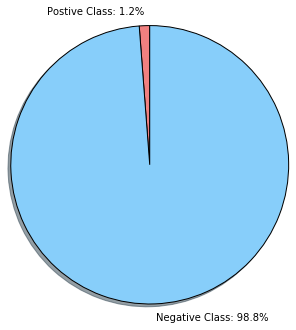
\includegraphics[width=1.0\linewidth]{figures/distribution_1.png}
        \caption{Classes are severely imbalanced}
        \label{fig:distribution_1}
    \end{subfigure}

   \begin{subfigure}[b]{0.9\linewidth}
        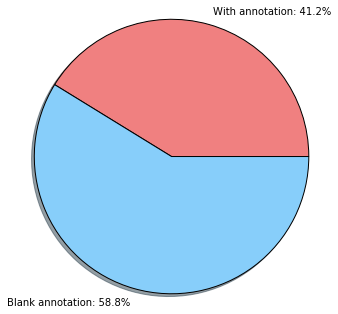
\includegraphics[width=1.0\linewidth]{figures/distribution_2.png}
        \caption{Majority of the images has blank annotations (i.e. no annotated brachial plexus)}
        \label{fig:distribution_2}
    \end{subfigure}

    \caption{Distribution of classes}
    \label{fig:distribution}
\end{figure}

\begin{figure*}[ht]
 \centering
  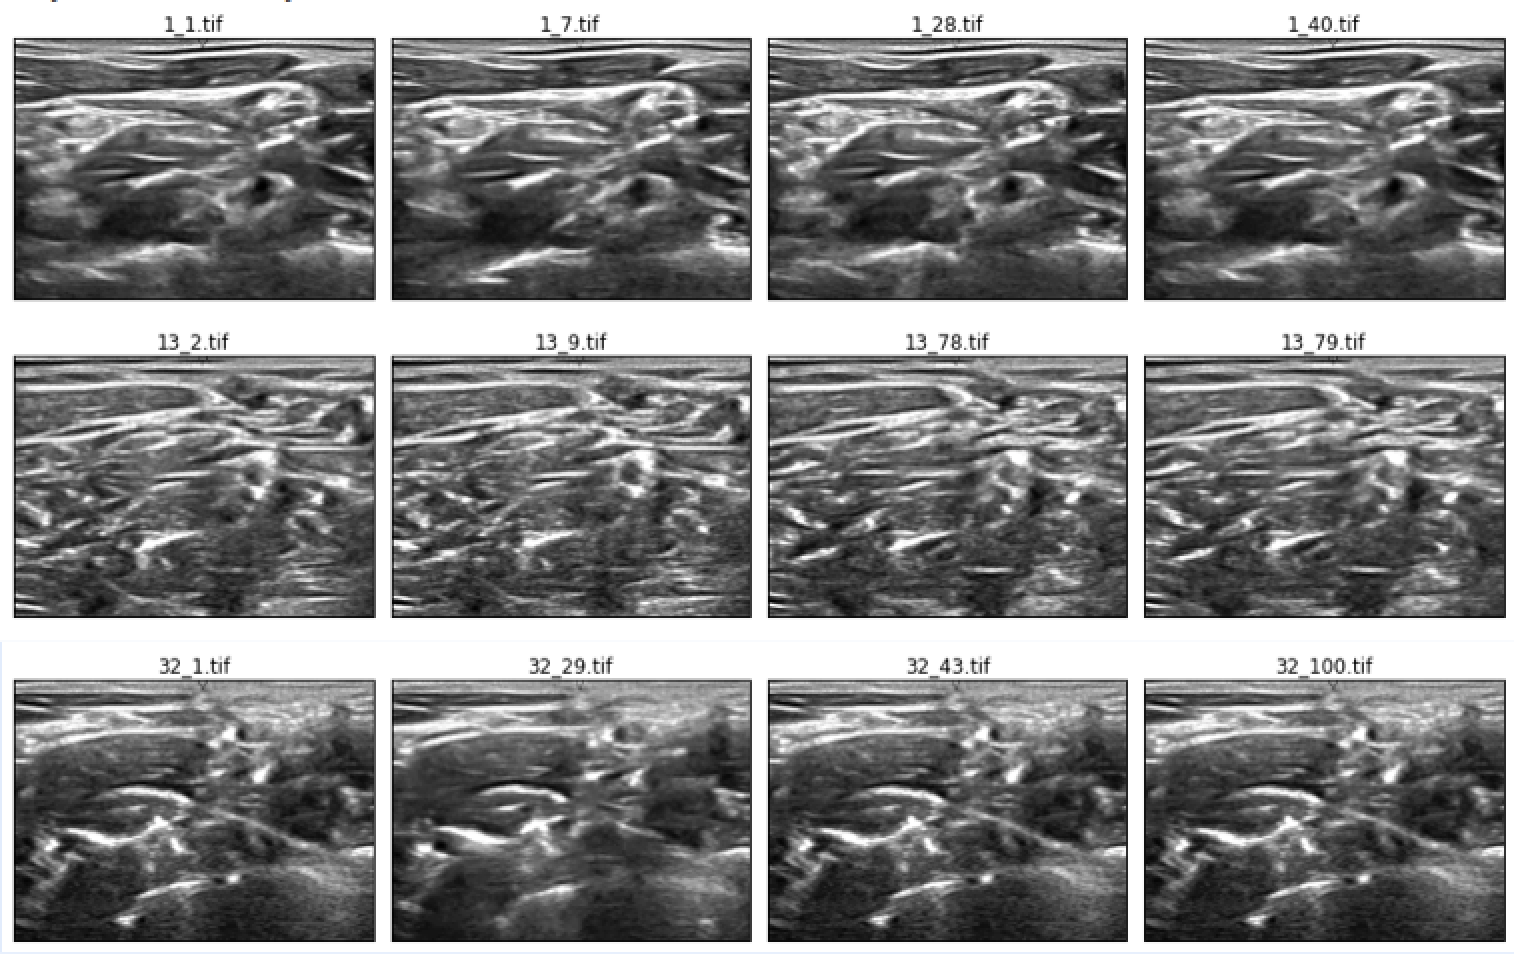
\includegraphics[width=0.8\linewidth]{figures/high_corr.png}
  \caption{
      High correlation of images. The file names have the format \textless patient\_id\_xxx.tif\textgreater . Images coming from the same patient ID are highly correlated. (NOTE: The images are not exactly the same.)
  }
  \label{fig:high_corr}
\end{figure*}

\begin{figure*}[ht]
 \centering
  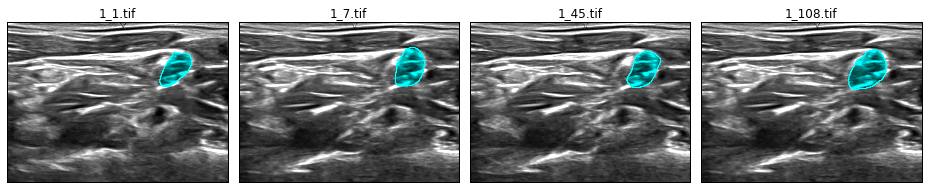
\includegraphics[width=0.8\linewidth]{figures/inaccurate_1.png}
  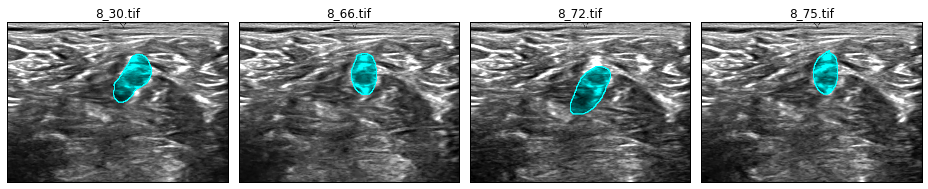
\includegraphics[width=0.8\linewidth]{figures/inaccurate_2.png}
  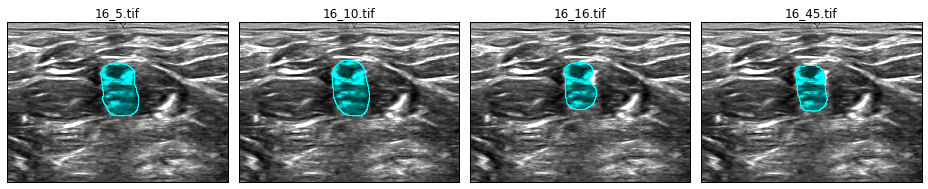
\includegraphics[width=0.8\linewidth]{figures/inaccurate_3.png}
  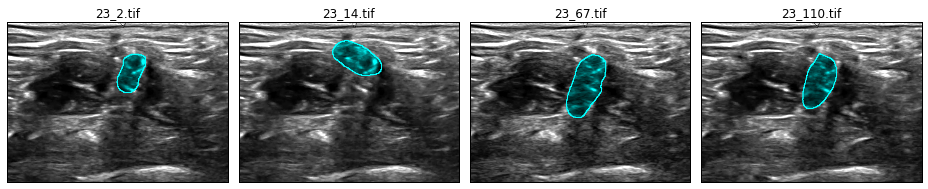
\includegraphics[width=0.8\linewidth]{figures/inaccurate_4.png}
  \caption{
      Similar images with varying annotations. Human-annotated training images have inaccurate annotations.
  }
  \label{fig:inaccurate}
\end{figure*}


\begin{figure*}[ht]
 \centering
  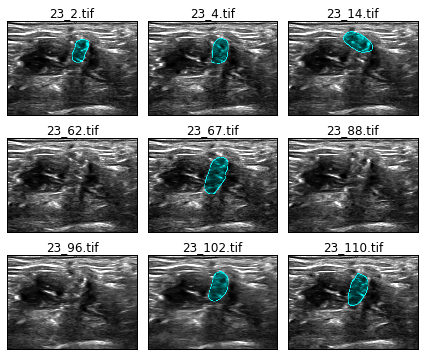
\includegraphics[width=0.7\linewidth]{figures/conflicting.png}
  \caption{
      Conflicting annotations. Very similar images have conflicting annotations. One image has BP while the other has none. These are human errors during manual annotation of the dataset.
  }
  \label{fig:conflicting}
\end{figure*}


\begin{figure*}[ht]
 \centering
  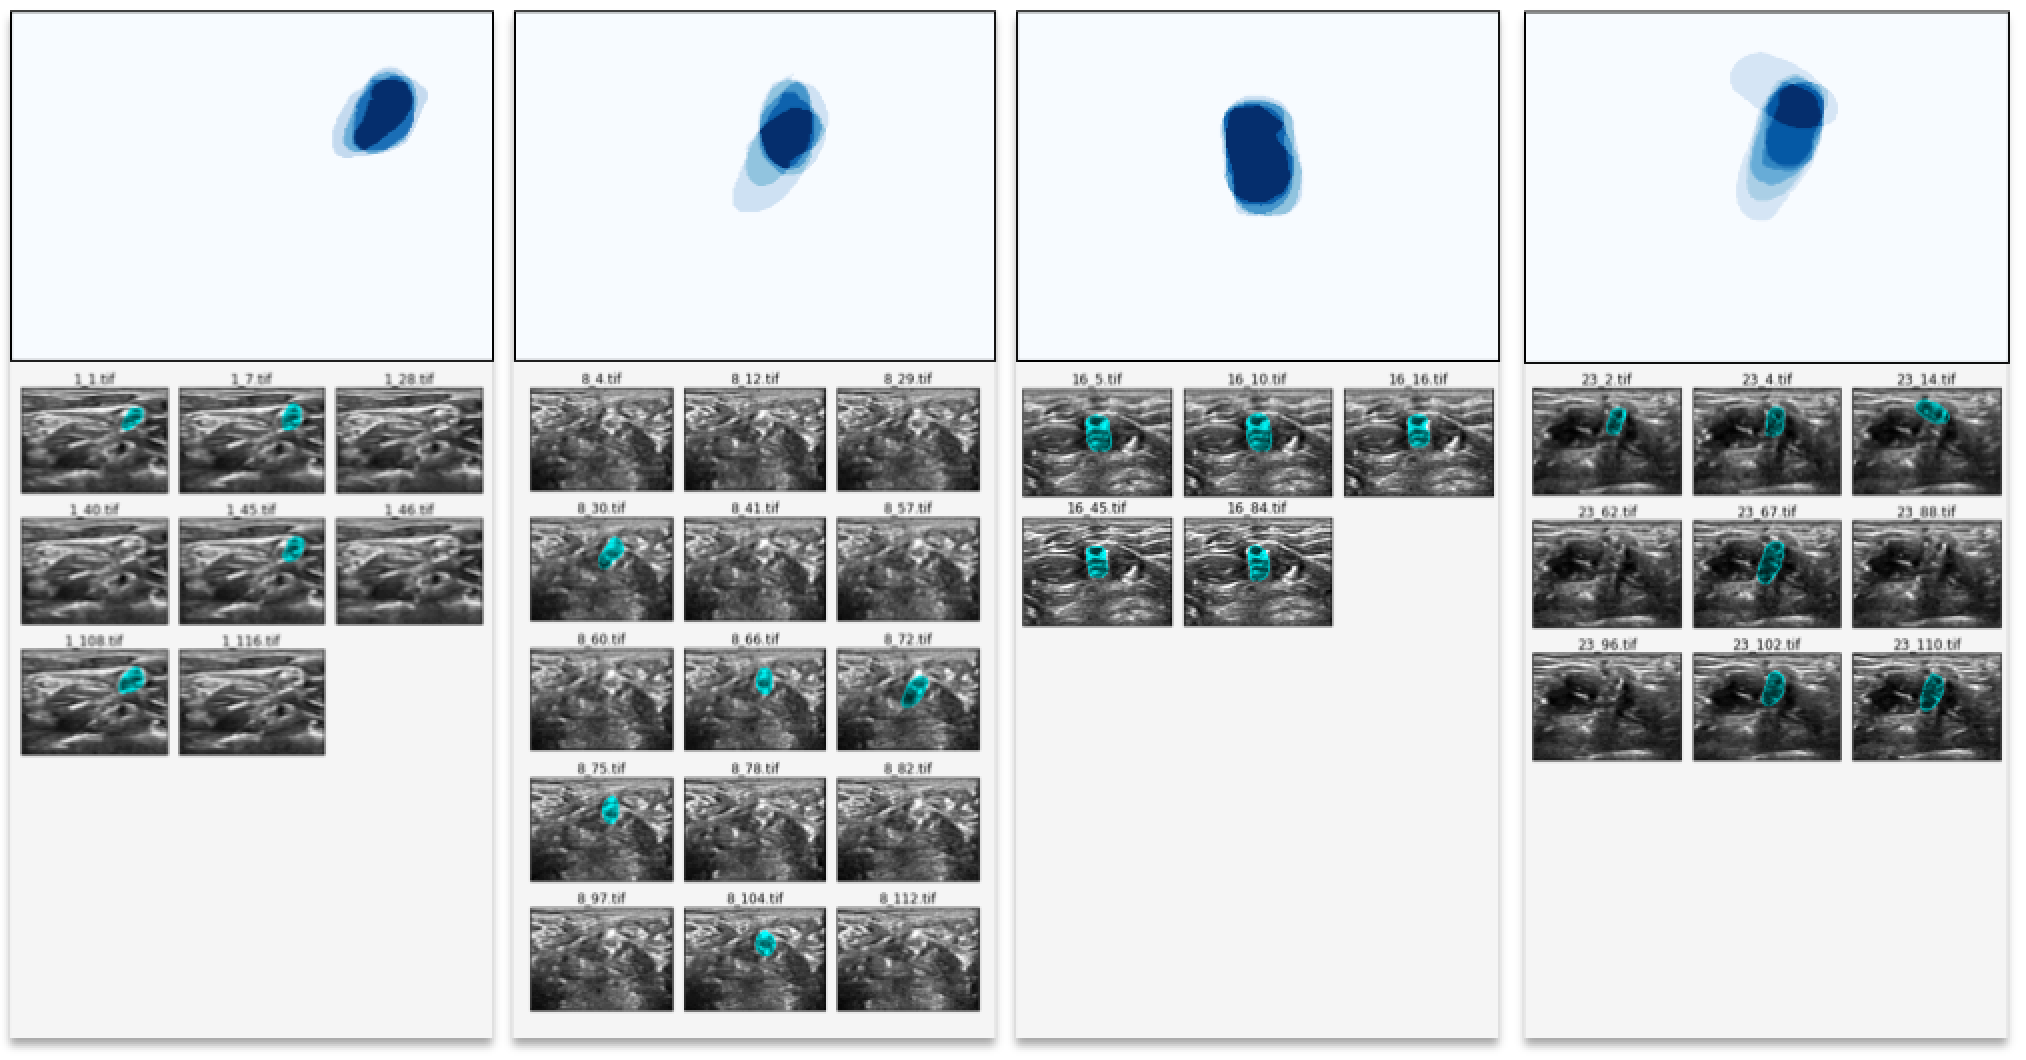
\includegraphics[width=1.0\linewidth]{figures/average_loc.png}
  \caption{
      Average annotations of similar images. Similar images have similar annotations, if present. The annotations do not exactly have the same shape, but they cover the same general area of the image and have common intersections.
  }
  \label{fig:average_loc}
\end{figure*}


\section{Analysis}
\subsection{Data Exploration}
There are 5,635 images for training and 5,508 images for testing. The images are gray scale with dimensions 580 x 420 pixels and are noisy. Training images have masks to indicate where the BP is present, while there is none for testing images. In the training images, only 2,323 images have positively identified the BP.
Groups of images are taken from the same patient.  Images that come from the same patient are highly correlated (see Figure \ref{fig:high_corr}).

The classes are severely imbalanced; consisting of $1.2\%$ positive class and $98.8\%$ negative class (see Figure \ref{fig:distribution}. This class imbalance is mitigated by using $F_1$ score.

There are inaccuracies in the annotations of the BP. There is no prefect ground truth or gold standard (see Figure \ref{fig:inaccurate}). There are very similar images but with conflicting annotations; one image has positively identified the BP, however the other has none (see Figure \ref{fig:conflicting}). There are also very similar images that have positive annotations, but the area where they are annotated differ in shape/area, although the annotations are located approximately in the same region (see Figure \ref{fig:average_loc}).



Where the BP is present in an image, the BP annotations has the following characteristics:

\centering
\begin{tabular}{l r}
Minimum size  &      2,684 pixels \\
Maximum size &    17,439 pixels \\
Average size   & 7,125.74 pixels \\
\end{tabular}





\bibliographystyle{icml2017}
\bibliography{main}


\end{document} 

